\section{Un modèle}
\label{sec:model}

Nous définissons maintenant le modèle \figref{model}, que les projets que nous allons analyser devrons respecter.
\begin{figure}[t]
  \centering
  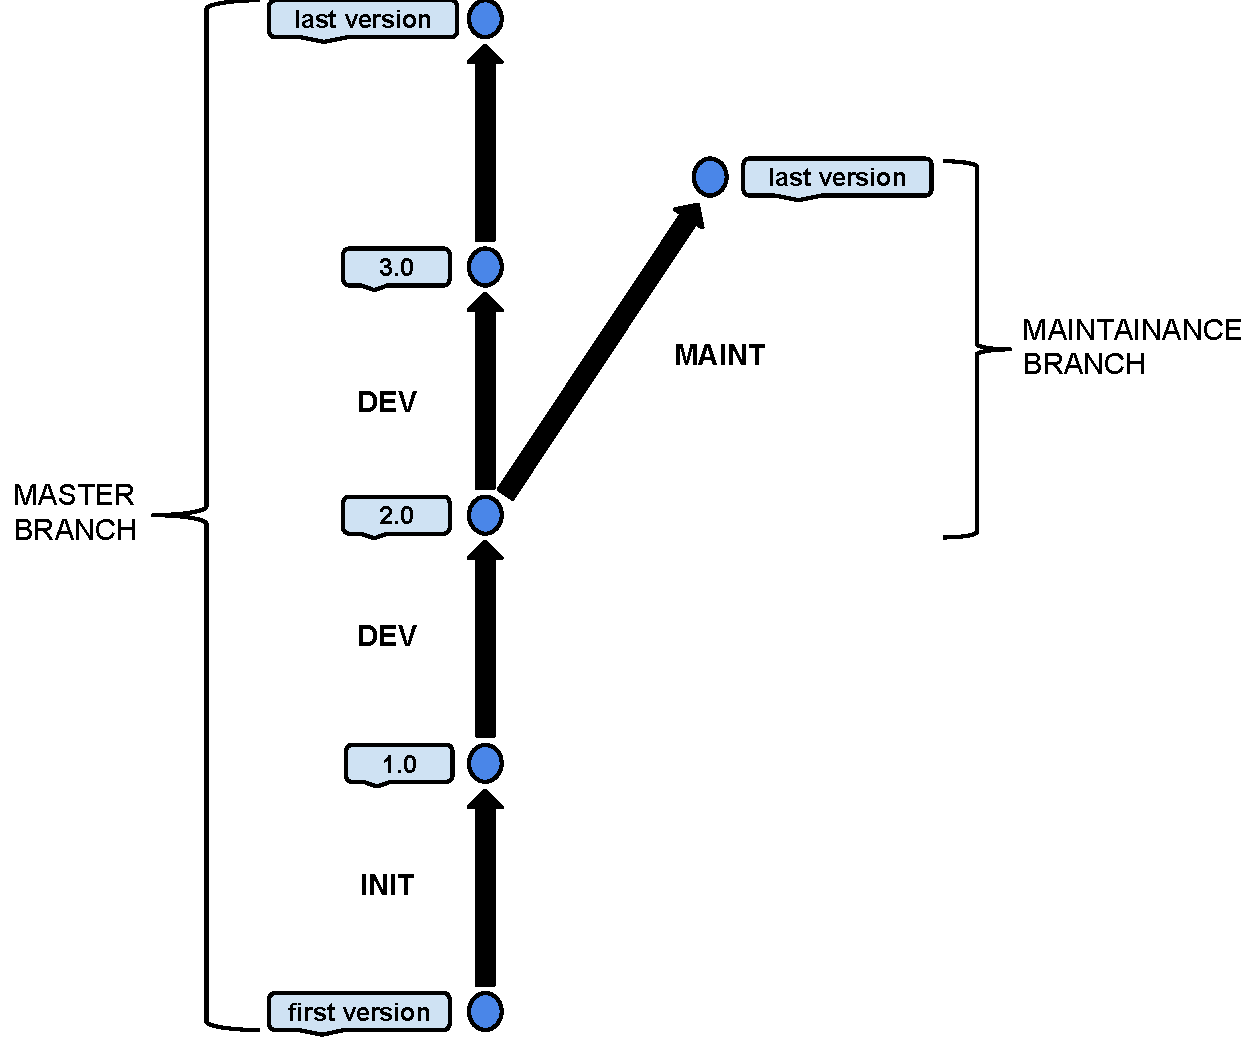
\includegraphics[scale=0.5]{data/figures/periods.pdf}
	\caption{Modèle d'architecture de dépot de code source}
	\label{fig:model}
\end{figure}
Celui ci modèle représente une architecture pour le dépôt de code source dérivé de l'architecture Git Flow.\\
Les projets de développement logiciel suivent généralement des phases distinctes durant leur cycle de vie. Habituellement une période de développement commence avant qu'une première release soit accessible aux utilisateurs, puis cette release est maintenue pendant qu'une autre se prépare et ainsi de suite.\\
Nous avons ainsi deux types de branches, les branches de maintenance et la branche master. Nous divisons les branches en périodes, c'est-à-dire en une séquence de commits, la branche master contient une période initiale (init) entre la première version du logiciel (incluse) et la première release, puis des périodes de développement (dev) entre chaque release. Chaque projet contient des releases majeures, qui correspondent à des points-clés du projet, des périodes susceptibles de contenir beaucoup de changements, et des releases mineures. On distingue les releases majeures des mineures par une augmentation significative du numéro de release. Par exemple $1.9-2.0$ pour Jquery, $3.7-4.0$ pour PHPUnit ou $0.13-1.0$ pour Rails. De l'autre côté les branches de maintenance sont divisées en périodes (maint) entre chaque release.\\
 

